\documentclass{article}
\usepackage{amsmath}
\usepackage{amssymb}
\usepackage{graphicx}
\usepackage{hyperref}
\usepackage[version=4]{mhchem}

\title{Example 21}
\date{}

\begin{document}
\maketitle

(1985 Yangzhou Math Contest, 1994 Canadian Mathematical Olympiad) Let \(A B C\) be an acute angled triangle. Let \(A D\) be the altitude on \(B C\), and let \(H\) be any interior point on \(A D\). Lines \(B H\) and \(C H\), when extended, intersect \(A C\) and \(A B\) at \(E\) and \(F\), respectively. Prove that \(\angle E D H=\angle F D H\).

Solution:
From \(A\) draw a line parallel to \(B C\). Extend \(C H, D F\), \(B E\), and \(D E\) to meet the line at \(Q, K, P\), and \(G\), respectively.\\
\centering
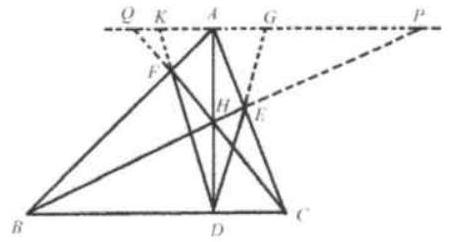
\includegraphics[width=\textwidth]{images/124(1).jpg}

We know that \(\triangle B D H \sim \triangle P A H . \frac{B D}{A P}=\frac{D H}{A H}\)\\
We know that \(\triangle C D H \sim \triangle Q A H . \frac{C D}{A Q}=\frac{D H}{A H}\)\\
From (1) and (2), we have: \(\frac{B D}{A P}=\frac{C D}{A Q}\) or\\
\(\frac{B D}{C D}=\frac{A P}{A Q}\)\\
\centering
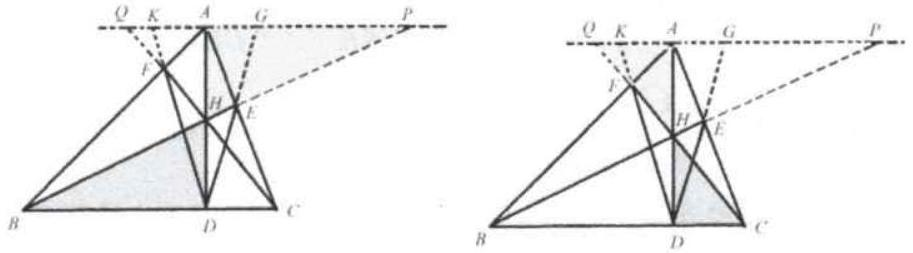
\includegraphics[width=\textwidth]{images/124(3).jpg}

We know that \(\triangle D C E \sim \triangle G A E . \frac{C D}{A G}=\frac{C E}{A E}\)

We know that \(\triangle B C E \sim \triangle P A E \cdot \frac{B C}{A P}=\frac{C E}{A E}\)


\begin{center}
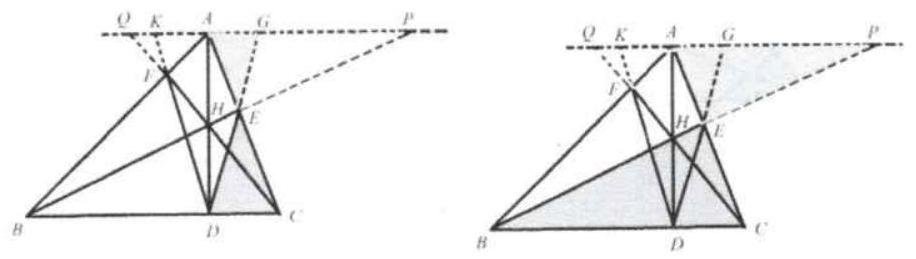
\includegraphics[width=\textwidth]{images/125(1).jpg}
\end{center}

From (4) and (5), we have: \(\frac{C D}{A G}=\frac{B C}{A P}\) or \(\frac{C D}{B C}=\frac{A G}{A P}\)

We know that \(\triangle B C F \sim \triangle A Q F . \frac{B C}{A Q}=\frac{B F}{A F}\)\\
We know that \(\triangle B D F \sim \triangle A K F . \frac{B D}{A K}=\frac{B F}{A F}\)\\
\centering
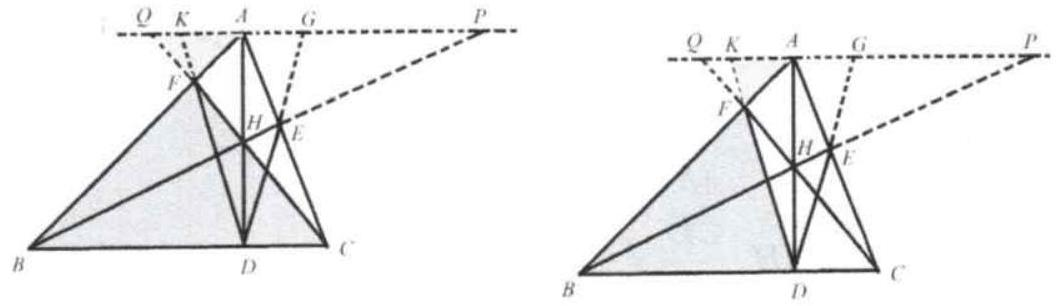
\includegraphics[width=\textwidth]{images/125.jpg}

From (7) and (8), we have: \(\frac{B C}{A Q}=\frac{B D}{A K}\) or \(\frac{B C}{B D}=\frac{A Q}{A K}\)\\
(3) \(\times(6) \times(9): \frac{A G}{A K}=1 \quad \Rightarrow \quad A G=A K\).

Since \(A D\) is the altitude, \(\triangle A D K\) and \(\triangle A D G\) are right triangles.\\
\(\triangle A D K \cong \triangle A D G(A G=A K . \angle D A K=\angle D A G, A D=A D)\)\\
Thus \(\angle E D H=\angle F D H\).


\end{document}
